% One-page slide figure (right side of Mingjia.pptx): a) training recipe, b) long-horizon, c) OOD control.
% Data: Tab. long_horizon and Tab. action_enhancement in 4_experiments.tex. Sized for a 4.5in x 4.4in slot.
\documentclass[border=3pt]{standalone}
% Shared style for PRISM figures. Compile with tectonic (XeTeX engine).
\usepackage{lmodern}
\usepackage{amssymb}
\usepackage{fontspec}
\setmainfont{Arial}
\setsansfont{Arial}
\usepackage{amsmath}
\usepackage{booktabs}
\usepackage{colortbl}
\usepackage{xcolor}
\usepackage{tikz}
\usetikzlibrary{arrows.meta,positioning,fit,calc,backgrounds,decorations.pathreplacing}
\usepackage{pgfplots}
\pgfplotsset{compat=1.18}

% PRISM template palette (sampled from the poster template)
\definecolor{prismdark}{HTML}{195A99}
\definecolor{prismmid}{HTML}{1D6FAA}
\definecolor{prismlight}{HTML}{9BB7DC}
\definecolor{prismpale}{HTML}{E8EFF8}
\definecolor{prismaccent}{HTML}{D9822B}
\definecolor{prismgray}{HTML}{6B7280}

\newcommand{\sz}[2]{\fontsize{#1}{#2}\selectfont}
\newcommand{\oursrow}{\rowcolor{prismpale}}
\pgfkeys{/pgf/number format/assume math mode=true}

\begin{document}
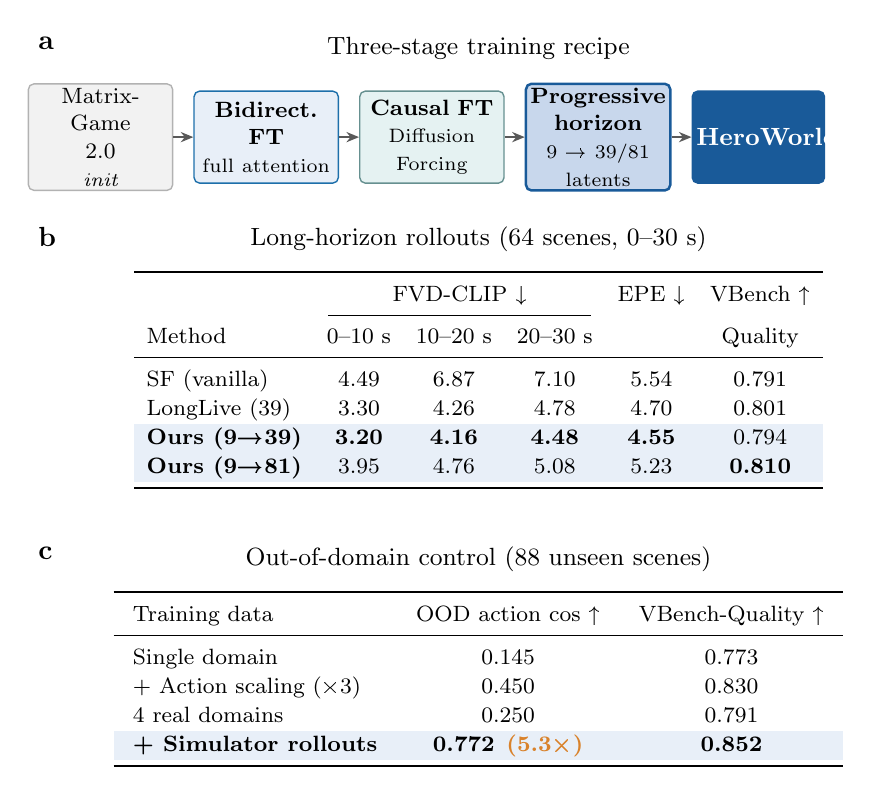
\begin{tikzpicture}[
  font=\sz{8.5}{10},
  >={Stealth[length=1.6mm,width=1.3mm]},
  stage/.style={rectangle, rounded corners=2pt, line width=0.5pt, minimum height=0.46in,
    text width=0.68in, inner sep=1.5pt, align=center},
  arr/.style={->, line width=0.7pt, draw=black!65},
  lbl/.style={anchor=north west, font=\sz{10}{12}\bfseries},
  ttl/.style={anchor=north, font=\sz{9.5}{11}},
]
% ---------- a ----------
\node[lbl] at (0,0) {a};
\node[ttl] at (2.25in,0) {Three-stage training recipe};
\begin{scope}[yshift=-0.55in]
\node[stage, fill=gray!10, draw=gray!60] (s0) at (0.36in,0) {Matrix-Game\\2.0\\{\sz{7}{8}\itshape init}};
\node[stage, fill=prismpale, draw=prismmid, right=0.1in of s0] (s1) {\textbf{Bidirect. FT}\\{\sz{7}{8} full attention}};
\node[stage, fill=teal!10, draw=teal!55!black!60, right=0.1in of s1] (s2) {\textbf{Causal FT}\\{\sz{7}{8} Diffusion Forcing}};
\node[stage, fill=prismlight!55, draw=prismdark, line width=0.9pt, right=0.1in of s2] (s3) {\textbf{Progressive}\\\textbf{horizon}\\{\sz{7}{8} 9 → 39/81 latents}};
\node[stage, fill=prismdark, draw=prismdark, text=white, font=\sz{9}{10}\bfseries, right=0.1in of s3, text width=0.62in] (s4) {HeroWorld};
\foreach \a/\b in {s0/s1,s1/s2,s2/s3,s3/s4} \draw[arr] (\a) -- (\b);
\end{scope}
% ---------- b ----------
\node[lbl] at (0,-0.95in) {b};
\node[ttl] at (2.25in,-0.95in) {Long-horizon rollouts (64 scenes, 0–30 s)};
\node[anchor=north] at (2.25in,-1.17in) {%
\sz{8.5}{10.5}\setlength{\tabcolsep}{4.5pt}%
\begin{tabular}{lccccc}
\toprule
 & \multicolumn{3}{c}{FVD-CLIP ↓} & EPE ↓ & VBench ↑ \\
\cmidrule(lr){2-4}
Method & 0–10 s & 10–20 s & 20–30 s & & Quality \\
\midrule
SF (vanilla)  & 4.49 & 6.87 & 7.10 & 5.54 & 0.791 \\
LongLive (39) & 3.30 & 4.26 & 4.78 & 4.70 & 0.801 \\
\oursrow \textbf{Ours (9→39)} & \textbf{3.20} & \textbf{4.16} & \textbf{4.48} & \textbf{4.55} & 0.794 \\
\oursrow \textbf{Ours (9→81)} & 3.95 & 4.76 & 5.08 & 5.23 & \textbf{0.810} \\
\bottomrule
\end{tabular}};
% ---------- c ----------
\node[lbl] at (0,-2.55in) {c};
\node[ttl] at (2.25in,-2.55in) {Out-of-domain control (88 unseen scenes)};
\node[anchor=north] at (2.25in,-2.77in) {%
\sz{8.5}{10.5}\setlength{\tabcolsep}{7pt}%
\begin{tabular}{lcc}
\toprule
Training data & OOD action cos ↑ & VBench-Quality ↑ \\
\midrule
Single domain             & 0.145 & 0.773 \\
+ Action scaling (×3)     & 0.450 & 0.830 \\
4 real domains            & 0.250 & 0.791 \\
\oursrow \textbf{+ Simulator rollouts} & \textbf{0.772} \,{\color{prismaccent}\textbf{(5.3×)}} & \textbf{0.852} \\
\bottomrule
\end{tabular}};
\end{tikzpicture}
\end{document}
